\documentclass[10pt,a4paper,landscape]{article}
\usepackage{multicol}
\usepackage{calc}
\usepackage{ifthen}
\usepackage[landscape]{geometry}
\usepackage{amsmath,amsthm,amsfonts,amssymb,mathtools}
\usepackage{color,graphicx}
\usepackage{hyperref}
\usepackage{listings}
\usepackage{underscore}
\usepackage{todonotes}

% Cheatsheet style
% Cheatsheet style

% This sets page margins to .5 inch if using letter paper, and to 1cm
% if using A4 paper. (This probably isn't strictly necessary.)
% If using another size paper, use default 1cm margins.
\ifthenelse{\lengthtest{\paperwidth = 11in}}
  % Then
  { \geometry{top=.5in,left=.5in,right=.5in,bottom=.5in} }
  % Else
  { \ifthenelse{\lengthtest{\paperwidth = 297mm}}
    {\geometry{top=1cm,left=1cm,right=1cm,bottom=1cm} }
    {\geometry{top=1cm,left=1cm,right=1cm,bottom=1cm} }
  }

% Turn off header and footer
\pagestyle{empty}

% Redefine section commands to use less space
\makeatletter
\renewcommand{\section}{\@startsection{section}{1}{0mm}%
                                {-1ex plus -.5ex minus -.2ex}%
                                {0.5ex plus .2ex}%x
                                {\color{darkred}\normalfont\large\bfseries}}
\renewcommand{\subsection}{\@startsection{subsection}{2}{0mm}%
                                {-1explus -.5ex minus -.2ex}%
                                {0.5ex plus .2ex}%
                                {\color{darkdarkred}\normalfont\normalsize\bfseries}}
\renewcommand{\subsubsection}{\@startsection{subsubsection}{3}{0mm}%
                                {-1ex plus -.5ex minus -.2ex}%
                                {1ex plus .2ex}%
                                {\normalfont\small\bfseries}}
\makeatother

% Define BibTeX command
\def\BibTeX{{\rm B\kern-.05em{\sc i\kern-.025em b}\kern-.08em
    T\kern-.1667em\lower.7ex\hbox{E}\kern-.125emX}}

% Don't print section numbers
\setcounter{secnumdepth}{0}

\setlength{\parindent}{0pt}
\setlength{\parskip}{0pt plus 0.5ex}

% Setting colors
\definecolor{lightgray}{rgb}{0.7,0.7,0.7}
\definecolor{lightergray}{rgb}{0.9,0.9,0.9}
\definecolor{darkblue}{rgb}{0.4,0.4,1}
\definecolor{darkred}{rgb}{0.9,0.2,0.2}
\definecolor{darkdarkred}{rgb}{0.6,0.0,0.0}
\definecolor{lightred}{rgb}{1,0.6,0.6}
\definecolor{lightgreen}{rgb}{0.6,1,0.6}
\definecolor{lightblue}{rgb}{0.6,0.8,1}
\definecolor{darkgreen}{rgb}{0.4,1,0.4}

% Set code listing style
\lstset {
    backgroundcolor=\color{lightgray},
    basicstyle=\ttfamily\scriptsize,
    breaklines=true,
}

\lstdefinestyle{bb}{
    backgroundcolor=\color{lightergray},
    frame=L,
    xleftmargin=\parindent,
}

% Remove `itemize` indentation
\usepackage{enumitem}
\setlist[itemize]{leftmargin=*}

% Set hyperlink style
\hypersetup{hidelinks}

% Enable figures
\newenvironment{colfig}
  {\par\medskip\noindent\minipage{\linewidth}}
  {\endminipage\par\medskip}

% Enable arg min/max math operators
\DeclareMathOperator*{\argmin}{arg\,min}
\DeclareMathOperator*{\argmax}{arg\,max}


% Shorthands
\renewcommand{\bf}[1]{\ensuremath{\mathbf{#1}}}
\newcommand{\E}{\mathrm{E}}
\newcommand{\Var}{\mathrm{Var}}
\newcommand{\Cov}{\mathrm{Cov}}
\newcommand{\balpha}{\boldsymbol\alpha}
\newcommand{\bbeta}{\boldsymbol\beta}
\newcommand{\bdelta}{\boldsymbol\delta}
\newcommand{\btheta}{\boldsymbol\theta}
\newcommand{\bPhi}{\boldsymbol\Phi}
\newcommand{\code}{\mathcal{C}}
\newcommand{\alphabet}{\mathcal{U}}

\pdfinfo{
  /Title (Machine Learning Cheat Sheet)
  /Creator (TeX)
  /Producer (pdfTeX 1.40.0)
  /Author (Dennis Meier)
  /Subject (Machine Learning cheatsheet)
  /Keywords (machinelearning, ml, bayes, regression, classification)
}

% -----------------------------------------------------------------------

\begin{document}
\title{Information Theory Cheat Sheet}

\raggedright
\footnotesize
\sffamily
\begin{multicols*}{4}

% multicol parameters
% These lengths are set only within the two main columns
%\setlength{\columnseprule}{0.25pt}
\setlength{\premulticols}{1pt}
\setlength{\postmulticols}{1pt}
\setlength{\multicolsep}{1pt}
\setlength{\columnsep}{2pt}

\begin{center}
\Large{\underline{Information Theory Cheat Sheet}}
\end{center}

% ----------
\section{Source Coding}
A source code $\code$ for a random variable $X$ is a mapping from the range of X to $D^*$, the set of finite-length strings of symbols from a D-ary alphabet.

\begin{colfig}
	\centering
	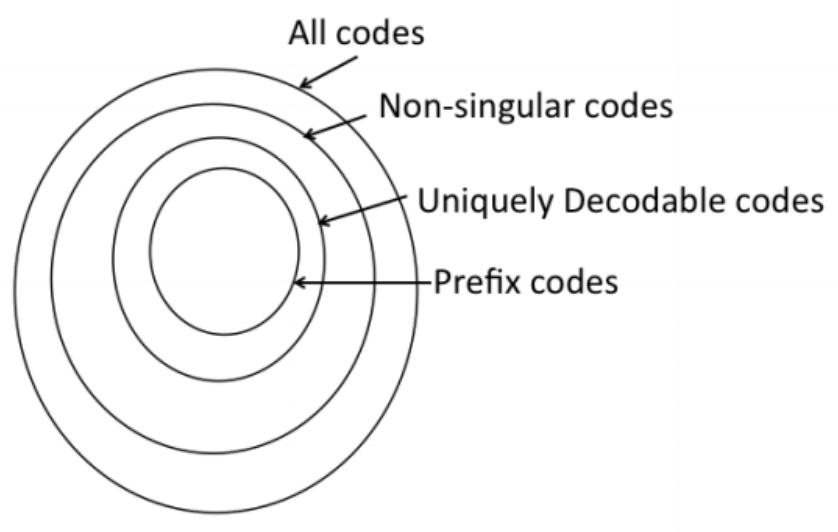
\includegraphics[width=\linewidth]{code-classes.png}
\end{colfig}

\subsection{Kraft's inequality}
$$\sum_{u \in \alphabet} 2^{-len(\code(u))} \leq 1$$

$\code$ prefix free $\implies$ Kraft

$\code$ uniquely decodable $\implies$ Kraft

$l(u)$ fullfills Kraft $\implies$ $\exists \ \code$, prefix free with $len(\code(u)) = l(u)$


\section{Entropy and co.}
\begin{colfig}
\centering
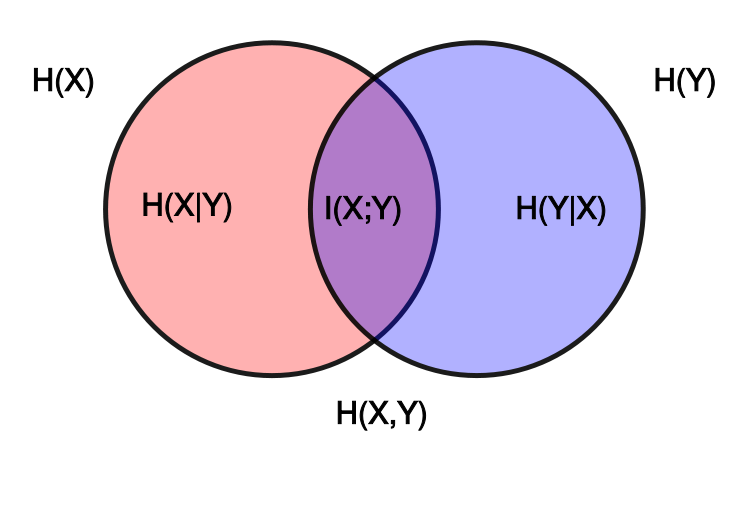
\includegraphics[width=\linewidth]{entropy-quantities-venn-diagram.png}
\end{colfig}

\subsection{Entropy}

$H(U) = \sum_u - P(u) \log_2(P(u)) = E[- \ln(P(U))]$

\subsubsection{Properties:}
\begin{itemize}
	\item $H(U) \leq \log | \alphabet |$ with equality if all elements in $\alphabet$ are equally probable.
	\item $H(U) \geq 0$ always.
	\item $H(U) \geq H(f(U))$
\end{itemize}

\subsection{Joint Entropy}
$H(X,Y) = H(X) + H(Y | X) = H(Y) + H(X | Y)$

\subsubsection{Properties:}
\begin{itemize}
	\item Joint increases entropy: $H(X, Y) \geq H(X)$ with equality iff $X$ and $Y$ are independent.
	\item $H(X,Y) \leq H(X) + H(Y)$
	\item Chain rule: $H(X, Y) = H(X) + H(Y | X)$
	\item General chain rule: $H(X_1, X_2, ..., X_n) = \sum_{i=1}^n H(X_i | X_1, ..., X_{i-1})$
\end{itemize}


\subsection{Conditional Entropy}

$H(U | V = v) = \sum_u - P(u | v) \log P(u | v)$

$H(U | V) = \sum_v P(v) H(U | V = v)$


\subsubsection{Properties:}
\begin{itemize}
	\item Conditioning reduces entropy: $H(U | V) \leq H(U)$
	\item Chain rule: $H( U | V) = H(U,V) - H(V)$
	\item If $X_i$ is a stationary stochastic process: $H(X_n | X^{n-1}) \leq H(X_i | X^{i-1})$ with $i \in 1, ..., n$
\end{itemize}


Expected codeword length: $E[len(\code(U))] < H(U) + 1$

\subsection{Mutual Information}
\begin{align*}
I(U; V) &= H(U) + H(V) - H(U,V)\\
		&= H(U) - H(U | V)\\
		&= H(V) - H(V | U)\\
		&= H(U,V) - H(U | V) - H (V | U)
\end{align*}

\subsubsection{Properties:}
\begin{itemize}
	\item Nonnegative: $I(U;V) \geq 0$ with equality if $U, V$ ar independent.
	\item Chain rule: $I(X,Y; Z) = I(X;Y) + I(Y; Z | X)$
	\item General chain rule for mutual Information: $I(X_1, ..., X_n; Y) = \sum_{i=1}^n I(X_i; Y | X_1, ..., X_{i-1})$
	\item Data processing inequality: $I(X,Y) \geq I(X, Z)$ if X, Y, Z form a markov-chain.
	\item Symmetric: $I(X;Y) = I(Y;X)$.
\end{itemize}

\subsection{Cross-Entropy}
$$ D(p || q) = \sum_x p(x) \log \frac{p(x)}{q(x)}$$

\section{Entropy Rate \& Typical Sets}
Entropy rate of a stochastic Process $\{X_i\}$ is

$$H(X_i) = \lim_{n \rightarrow \infty} \frac{1}{n} H(X_1, X_2, ..., X_n)$$

\subsection{Asymptotic Equpartition Property}
Information Theory's analog to the law of large numbers: If $X_1, X_2, ...$ are i.i.d. $\sim p(x)$, then
$$ - \frac{1}{n} \log p(X_1, X_2, ..., X_n) \rightarrow H(X) \text{ in probability}$$

Or alternatively,

$$ p(X_1, X_2, ..., X_n) \rightarrow 2^{-n H}$$

\subsection{Typcial Set}
The typical set $T_\epsilon$ is the set of sequences $(x_1, x_2, ..., x_n) \in \alphabet^n$ such that:

$$p(x_1, x_2, ..., x_n) = 2^{-n(H(X) \pm \epsilon)}$$

\subsubsection{Properties of the typical set:}
\begin{itemize}
	\item Has probability nearly 1: $P(T_\epsilon) > 1 - \epsilon$
	\item All elements in $T_\epsilon$ are nearly equiprobable (with probability as given above)
	\item The number of elements in $T_\epsilon$ is nearly $2^{nH}$
\end{itemize}


\section{Utilities}
$\log(x) \leq 1 + x$

$\lceil x \rceil < 1 + a$

$E[Z] = \sum_{n=0}^{\infty} Pr[Z > n]$

Jensen's inequality for convex functions $f$: $ E[f(X)] \geq f(E[X])$

$a^b = 2^{ b \log a}$


\end{multicols*}
\end{document}
